\chapter{Aircraft Design Case Studies}

As indicated in Table \ref{tab:paradigm_comparison}, the main benefit of the proposed code transformations paradigm is to achieve runtime performance comparable to specialized methods, but without sacrificing ease-of-use and mathematical flexibility. Because this value proposition hinges on this usability, it becomes especially important to demonstrate the effectiveness of the proposed paradigm in real-world engineering applications.

In order to support this goal, Chapter \ref{chapter-code-transformations} introduced an example framework, AeroSandbox, which implements the proposed code transformations paradigm. AeroSandbox was developed using an iterative ``spiral development process'', which is depicted in Figure \ref{fig:spiral}. In short, at every step of the development process, a symbiotic bidirectional relationship between the framework and the case studies was maintained; the goal of this was to simultaneously ask and answer two questions:

\begin{enumerate}[noitemsep]
    \item Using the capabilities of this design framework, how can we improve this airplane and gain practical insight into the specific design space at hand?
    \item Based on this airplane case study, what broadly-applicable user needs and workflows can we identify, and how can we improve our design framework accordingly?
\end{enumerate}

\begin{figure}[H]
    \centering
    \includesvg[width=0.8\textwidth]{../figures/spiral.svg}
    \caption{The iterative spiral development process used to develop AeroSandbox, where applied use and framework development are intertwined. The aircraft in the figure is a visualization output using the AeroSandbox geometry stack, and depicts the hydrogen-fueled aircraft from the case study of Section \ref{sec:hydrogen}.}
    \label{fig:spiral}
\end{figure}

Over the development history of AeroSandbox, this spiral process was iterated upon multiple times, with each iteration resulting in a more refined and capable framework. This chapter presents a few vignettes of the various case studies that were used to develop AeroSandbox, which provides a fruitful opportunity to discuss the practical capabilities enabled by a code transformations MDO paradigm. It is important to emphasize that, although the aircraft design case studies presented in this chapter are fascinating real-world problems, the main intended intellectual contribution of this portion of the thesis is not the design of these specific aircraft (or even the example framework itself\footnote{MDO frameworks naturally come and go over the years as new opportunities in scientific computing and programming languages emerge. It is not the author's intent or expectation that AeroSandbox be the ``end-all'' framework for aircraft design. Rather, it is a proof-of-concept implementation that aims to demonstrate the potential utility of one possible framework approach for readers interested in building a future framework.}). Instead, the deeper goal is to introduce a principled paradigm for building engineering design optimization frameworks. Because of this, complete detailed enumeration of all modeling assumptions for specific problems is omitted in this chapter for brevity; however, both references to literature discussing these details and links to the raw source code itself are provided for most case studies, for the interested reader.


\section{Simple Aircraft Design Problem}
\label{sec:simpleac}

\begin{quote}
    \emph{This section includes content adapted from the author's prior work} \cite{sharpe_aerosandbox_2021}.
\end{quote}

A first simple aircraft design problem, called \emph{SimpleAC}, is included here to show what design code might look like in code transformations framework at the early stages of conceptual aircraft sizing. At this ``napkin-math'' stage, the main analyses (e.g., aerodynamics, structures, propulsion) can be cleanly expressed in simple analytical expressions, and the optimizer fulfills the role of closing the sizing loop. Because of this, this problem is simple enough to include both the complete problem statement and the complete solution code directly here, which is useful for readers interested in observing the mapping between these. This design problem itself was proposed by Hoburg \cite{hoburg} and is reproduced (with slight modifications) by both Ozturk \cite{Ozturk2018} and Kirschen \cite{kirschen}. It is restated here in full form:

\begin{example}
    \textbf{Simple Aircraft (SimpleAC)}
    \begin{mini}
        |l|
            {\AR, S, V, W, C_L, W_f, V_\text{f, fuse}}{W_f}
            {}{}
        \addConstraint{W \geq W_0 + W_w + W_f}
        \addConstraint{W_0 + W_w + \frac{1}{2} W_f \leq L_\text{cruise}}
        \addConstraint{W \leq L_\text{takeoff}}
        \addConstraint{W_f \geq \text{TSFC} \cdot t_\text{flight} \cdot D}
        \addConstraint{V_\text{f, wing} + V_\text{f, fuse} \geq V_f}
        \label{eq:simpleac}
    \end{mini}
    \begin{eqexpl}
        \item{$D$} Cruise drag
        \item{$\AR$} Wing aspect ratio (here, the wing is assumed to be rectangular)
        \item{$S$} Wing area
        \item{$V$} Cruise airspeed
        \item{$W$} Total weight
        \item{$C_L$} Cruise lift coefficient
        \item{$W_f$} Fuel weight
        \item{$V_\text{f, fuse}$} Volume of fuel in fuselage
    \end{eqexpl}

    \noindent
    We are also given the following physics models:

    \begin{itemize}[noitemsep]
        \item The chord $c = \sqrt{S / \AR}$, from geometric relations.
        \item The drag $D = \frac{1}{2} \rho V^2 C_D S$
        \item The drag coefficient $C_D = \frac{\mathrm{CDA}_0}{S} + k C_f \frac{S_\text{wet}}{S} + \frac{C_L^2}{\pi \AR e}$
        \begin{itemize}[noitemsep]
            \item $C_f = 0.074 \cdot \text{Re}^{-0.2}$, the Schlichting turbulent flat plate boundary layer model
            \item $\text{Re} = \frac{\rho V c}{\mu}$
        \end{itemize}
        \item The cruise lift $L_\text{cruise}=\frac{1}{2}\rho V^2 C_L S$
        \item The takeoff lift $L_\text{takeoff}=\frac{1}{2}\rho V_\text{min}^2 C_{L, \text{max}} S$
        \item The wing weight $W_{\text{wing}}= W_\text{w, structural} + W_\text{w, surface}$
        \begin{itemize}[noitemsep]
            \item $W_\mathrm{w,\ structural} = W_\text{w, c1} \cdot \frac{N \AR^{1.5} \sqrt{W_0 W S}}{\tau}$
            \item $W_\mathrm{w,\ surface} = W_\text{w, c2} \cdot S$
        \end{itemize}
        \item The aircraft's endurance $t_\text{flight} = \text{Range} / V$
        \item The fuselage drag area scales with fuel volume as $\text{CDA}_0 = V_\text{f, fuse} / (10\ \si{\meter})$
        \item The total fuel volume $V_f = \frac{W_f}{g\rho_f}$
        \item The fuel volume in the wing $V_\text{f, wing} = 0.03 S^{1.5} \AR^{-0.5} \tau$
    \end{itemize}

    \begin{eqexpl}
        \item {$g$} $9.81\ \si{\meter/\second\squared}$, Earth gravity.
        \item {$\rho_f$} $817\ \si{\kg/\meter\cubed}$, the density of fuel.
        \item {$\text{Range}$} $1000\ \si{\kilo\meter}$, the aircraft mission range.
        \item {$\text{TSFC}$} $0.6\ \si{\per\hour} = 1.67 \times 10^{-4}\ \si{\per\second}$, the thrust-specific fuel consumption.
        \item {$k$} $1.17$, the form factor.
        \item {$e$} $0.92$, the Oswald efficiency factor.
        \item {$\mu$} $1.775 \times 10^{-5}$ \si{\kg\per\meter\per\second}, the sea-level dynamic viscosity of air.
        \item {$\rho$} $1.23\ \si{\kg/\meter\cubed}$, the sea-level density of air.
        \item {$\tau$} $0.12$, the airfoil thickness-to-chord ratio.
        \item {$N$} $3.3$, the ultimate load factor.
        \item {$V_\text{min}$} $25\ \si{\meter/\second}$, the takeoff airspeed.
        \item {$C_{L, \text{max}}$} $1.6$, the takeoff lift coefficient.
        \item {$S_\text{wet}/S$} $2.075$, the wetted area ratio.
        \item {$W_0$} $6250 \si{\newton}$, the aircraft weight excluding the wing and fuel.
        \item {$W_\text{w, c1}$} $2 \times 10^{-5}\ \si{\per\meter}$, a wing weight coefficient.
        \item {$W_\text{w, c2}$} $60\ \si{\Pa}$, another wing weight coefficient.
    \end{eqexpl}

\end{example}

This design problem can be translated from the formulation above into the solution code, which is given in Appendix \ref{sec:simpleac-code}. Notably, the code of this problem is essentially a 1:1 translation of the problem statement into Python code, with almost zero additional boilerplate code required to set up this problem beyond the raw physics models and constants definitions. In fact, the code version of this problem is actually shorter on-the-page than the natural-language problem statement itself. This conciseness is a good approximate measure of the framework's usability, since it allows the user to focus on the problem physics and mathematical formulation, rather than the numerical mechanics of the optimization process.

The code given in Appendix \ref{sec:simpleac-code} converges to a solution in 14 iterations, with a median runtime\footnote{Measured on a laptop a Ryzen 7 5800H CPU. Measures end-to-end wall-clock runtime, including problem formulation (i.e., tracing, in Python), optimization (via IPOPT, in C++), and function evaluation (i.e., on the CasADi VM, in C++).} of 18 milliseconds. This is effectively-instantaneous for a human user, and this speed combined with the conciseness of the code gives the user great flexibility to explore the design space. The results of this AeroSandbox solve are shown in Table \ref{tab:simpleac}, and are consistent with the results of Ozturk \cite{ozturk_conceptual_2018}.

\begin{table}[H]
    \centering
    \caption{Solution of SimpleAC (Eq. \ref{eq:simpleac}), found with AeroSandbox.}
    \label{tab:simpleac}
    \begin{tabular}[t]{ll}
        \toprule
        Figure of Merit                            & Optimal Value             \\
        \midrule
        Fuel weight $W_f$                          & 937.8 \si{\newton}        \\
        Aspect ratio $\AR$                         & 12.10                     \\
        Wing area $S$                              & 14.15 \si{\meter\squared} \\
        Cruise airspeed $V$                        & 57.11 \si{\meter/\second} \\
        All-up weight $W$                          & 8705 \si{\newton}         \\
        Cruise lift coefficient $C_L$              & 0.2901                    \\
        Fuel volume in fuselage $V_\text{f, fuse}$ & 0.0619 \si{\meter\cubed}  \\
        \bottomrule
    \end{tabular}
\end{table}

% TODO elaborate


\section{MIT Firefly Micro-UAV}
\label{sec:firefly}

\subsection{Vehicle Overview}

One of the first aircraft design case studies used to develop AeroSandbox was the \emph{MIT Firefly}, a small tube-stowed, rocket-propelled, transonic micro-UAV. The concept of operations of this air vehicle is summarized in Figure \ref{fig:firefly_conops}. Firefly is designed to be deployed in-flight from a host aircraft, launching from a small standardized canister. This requires that the aircraft fit within a $70 \times 70 \times 480$ mm box in its stowed configuration, but the requirements admit the option of unfolding the vehicle into a flight configuration immediately after launch. After launch, the air vehicle is required to maintain an airspeed of at least Mach 0.8 for at least 60 seconds, without loss of altitude; this is termed the ``dash phase''. After the dash phase, the vehicle continues to fly in a ``glide phase'' until it runs out of both propulsive energy and altitude, at which point it performs a controlled crash landing. During this glide phase, there are no airspeed or other trajectory restrictions. The objective of the vehicle design is to maximize the \emph{total mission range}, including both the dash and glide phases.

\begin{figure}[H]
    \centering
    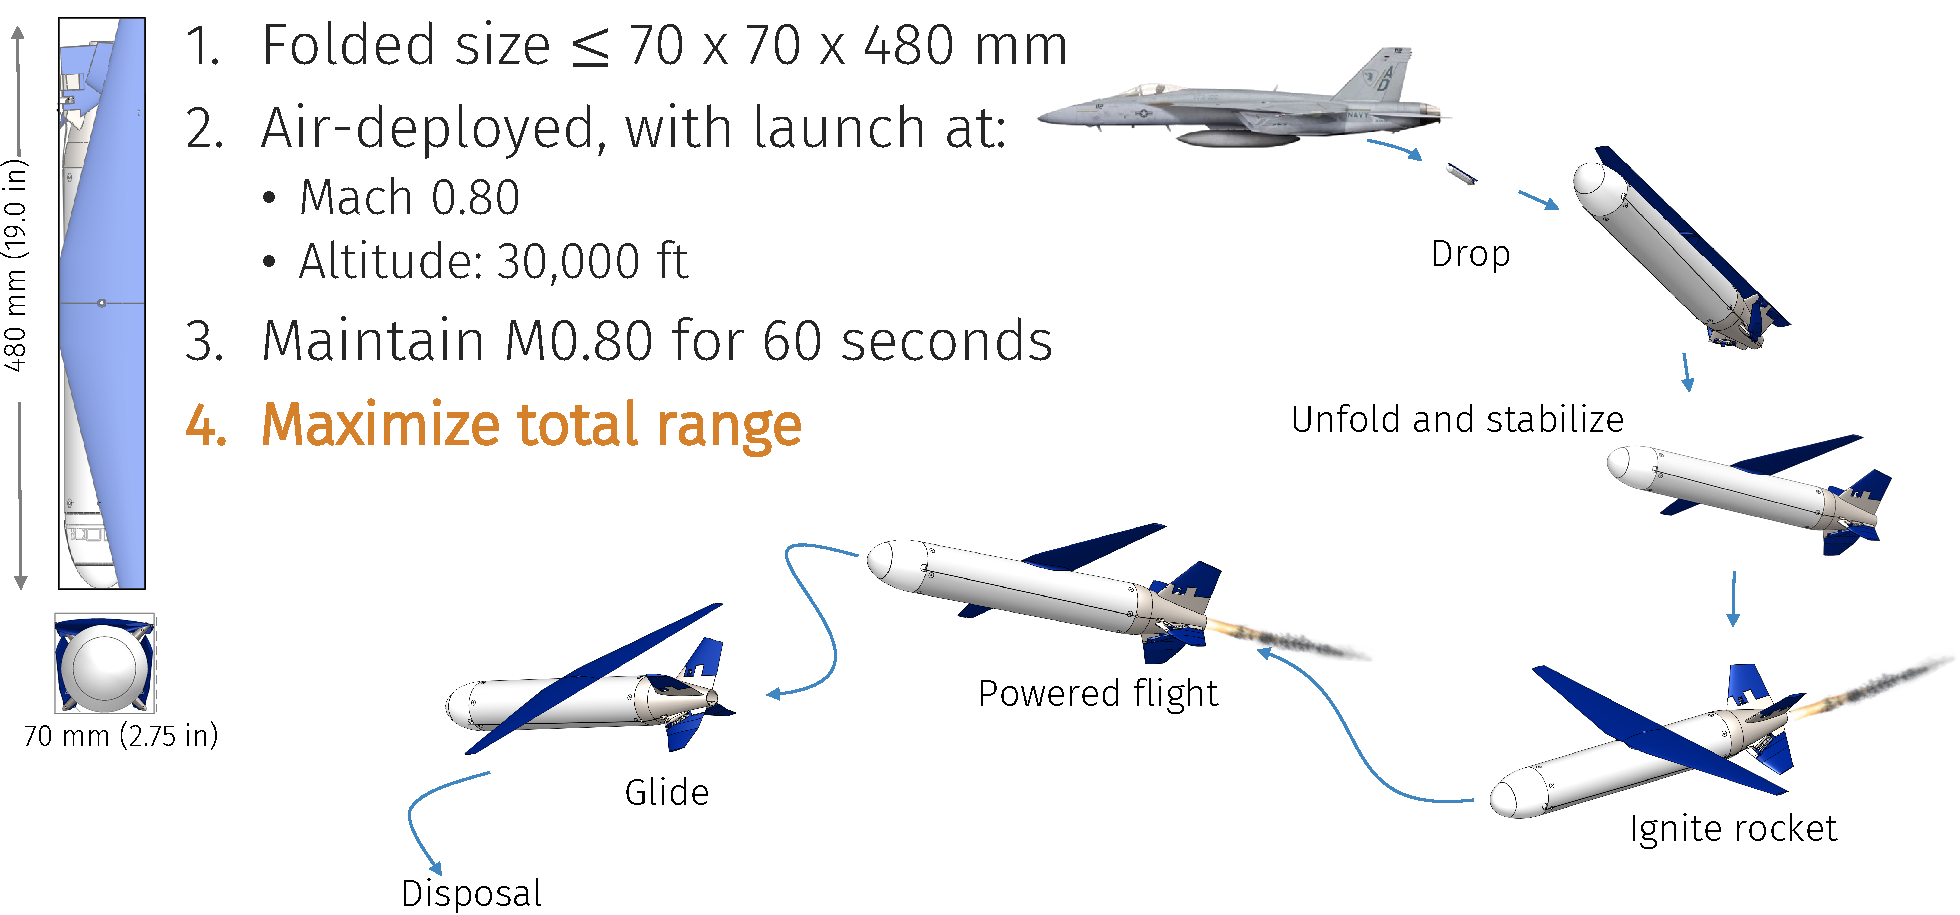
\includegraphics[width=\textwidth]{../figures/firefly_conops-crop.pdf}
    \caption{Concept of operations for the MIT Firefly UAV, adapted from Vernacchia \cite{vernacchia_development_2020}. CAD renders prepared by Julia Gaubatz \cite{gaubatz_design_2024}. F/A-18 image reproduced from McDonnell Douglas.}
    \label{fig:firefly_conops}
\end{figure}

As explained by Vernacchia \cite{vernacchia_development_2020}, Firefly aims to fill a previously-unexplored ``small and fast gap'' in the aircraft design space, with sustained cruise speeds of Mach 0.8 and a gross weight of 2.2 kg\footnote{For comparison: most air vehicles at this size scale are propeller-driven and fly at roughly Mach 0.2 or less. Most air vehicles capable of this sustained speed have gross weights at least an order of magnitude larger.}.

\begin{figure}[h]
    \centering
    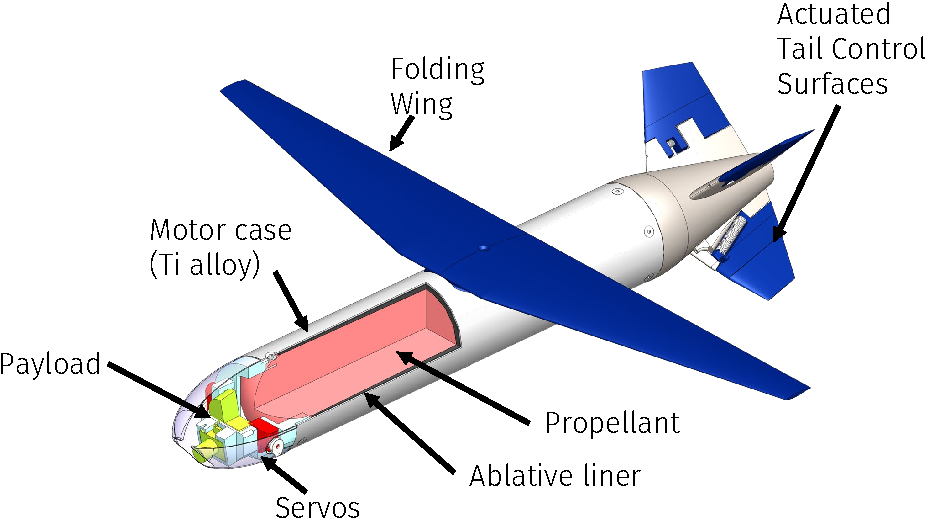
\includegraphics[width=\textwidth]{../figures/firefly_cutout-crop.pdf}
    \caption{Cutout-view of MIT Firefly, showing various unique features. CAD render prepared by Julia Gaubatz \cite{gaubatz_design_2024}.}
    \label{fig:firefly_cutout}
\end{figure}

Before even beginning the computational design process, we can observe some high-level design drivers from first principles. First, the vehicle is relatively insensitive to mass, which contrasts strongly with most aircraft design problems. This is because of a few reasons:
\begin{itemize}[noitemsep]
    \item The vehicle is air-launched at the dash speed and altitude, which means that no additional propulsive energy need be expended to reach this state. Although some of this initial kinetic energy is lost to drag during the initial stabilization transient upon deployment\footnote{and added mass tends to increase the moments of inertia, which slows down the short-period flight dynamics mode}, this is a relatively minor effect.
    \item During the dash phase, the freestream dynamic pressure is extremely high relative to the vehicle's projected area. In fact, were it not for the glide phase, the folding wing shown in Figure \ref{fig:firefly_conops} could be discarded, and body lift alone would be easily produce sufficient aerodynamic lift. Because of where this vehicle operates on the drag polar during the dash phase, the drag force is relatively insensitive to lift, and hence, vehicle weight.
    \item During the glide phase, the vehicle can be trimmed to any preferred airspeed, and naturally, the range-maximizing trajectory will have the aircraft fly at the best-glide speed. The glide ratio is essentially invariant to vehicle mass\footnote{barring some slight Reynolds number effects due to best-glide speed change, which are higher-order effects.}, so the range is also relatively insensitive to vehicle weight.
\end{itemize}

Because of this insensitivity to mass and the focus on total range, one can predict that the major design drivers for Firefly should essentially distill into the following:
\begin{itemize}[noitemsep]
    \item To maximize range during the dash phase: a) pack as much useful propulsive energy into the specified volume as possible, such that this dash phase can be sustained as long as possible and b) reduce drag, even at the expense of lift.
    \item To maximize range during the glide phase: achieve the highest $L/D$ ratio possible.
\end{itemize}

This first-principles design driver calling for the highest-possible volumetric energy storage naturally leads to hydrocarbon fuels\footnote{as opposed to electric batteries}. To achieve reasonable propulsive efficiency at Mach 0.8, the practical propulsion architectures are either a turbine engine or a rocket engine (which may be solid, liquid, or hybrid); tradeoffs are discussed by Vernacchia \cite{vernacchia_development_2020}. In short, a solid rocket engine requires far less ``volume overhead'' to be spent on the engine itself than any other option, especially at this size scale\footnote{Though first-principles physics favor a solid rocket, implementing this comes with some challenges. A particularly interesting one is how to slow down the burn such that the total impulse can be spread across a long enough duration. Vernacchia \cite{vernacchia_development_2020} and Mathesius \cite{mathesius_integrated_2023, mathesius_firefly_2019} explore a mix of clever chemical and physical strategies to achieve this.}. This allows the most possible volume to be spent on energy-rich propellant.

These design drivers also allow one to easily foresee that volume allocations will come at a premium when designing Firefly: expanding the volume available for propellant will inevitably result in fuselage shapes that generate more wave drag at the M0.8 dash condition\footnote{because these higher-volume shapes are blunter, and hence cause a deeper low-pressure spike resulting in stronger shock formation}. This sets the stage for an interesting multidisciplinary design optimization problem, where these coupled relationships can be explored further.

\subsection{MDO Problem Formulation}
\label{sec:firefly-mdo}

The design of Firefly is formulated as a combined vehicle-and-trajectory optimization problem, as these two are inextricably linked. The trajectory is represented via a predetermined number of discrete points in time (roughly $N=200$), which are connected via a direct collocation method\footnote{A introduction to the math representing the dynamics here is given by Kelly \cite{kelly_introduction_2017}.}. This is depicted in Figure \ref{fig:firefly_time_discretization}.

Because the flight physics fundamentally change between dash and glide phases (as the rocket motor no longer produces thrust after this point, and some aerodynamic changes regarding base drag occur), Firefly is inherently a multi-phase dynamics problem. Accordingly, the discretized dynamics are partitioned into two phases. Critically, to maintain $C^1$-continuity (and hence, optimization friendliness), we employ a strategy that we call \emph{stretchy time} that ensures that any given discretization node never crosses this phase boundary, as this would cause a discontinuous change in the problem physics. In this strategy, the time values corresponding to phase transitions (e.g., when rocket motor burnout occurs; when the vehicle contacts the ground and terminates the mission) are free variables in the optimization problem. In contrast, the time values corresponding to intermediate points have their relative spacing within a phase fixed \emph{a priori}. (In this case, this is done with ``cosine-spaced'', also called Chebyshev node, relative positions in time.) Points in time that fall exactly on a phase boundary are included in both phases, with a zero-time-difference collocation constraint that stitches the two phases together; this adds a few degrees of freedom but greatly simplifies indexing.

\begin{figure}[H]
    \centering
    \includesvg[width=0.7\textwidth]{../figures/firefly_time_discretization.svg}
    \caption{``Stretchy time'' time discretization strategy used for the MIT Firefly MDO problem and other multi-phase combined-vehicle-and-dynamics optimization problems.}
    \label{fig:firefly_time_discretization}
\end{figure}

The physics formulation of the optimization problem can be summarized as follows:

\begin{example}
    \textbf{MIT Firefly MDO Problem Formulation}

    \begin{itemize}
        \item \textbf{Objective Function}: Maximize the total mission range, defined as the sum of the dash and glide phases.

        \item \textbf{Design Variables} (in total, 3,910 variables):
        \begin{itemize}
            \item A series of trajectory design variables, including downrange distance, altitude, airspeed, flight path angle, angle of attack, and control surface deflections. Note that this parameterization a) is two-dimensional, representing the trajectory in range-altitude space and b) makes a quasi-steady assumption\footnote{using the definition from Drela \cite{drela_flight_2013}}, which essentially assumes that the short-period mode is much faster than the meaningful trajectory dynamics\footnote{Equivalent ways to state this are that we assume the vehicle an instantaneously trim to a desired angle of attack, or that the nondimensionalized angular rates (e.g., $\bar{p}, \bar{q}, \bar{r}$) are very small.}.

            \item Various other time-dependent variables, such as the instantaneous fuel mass, chamber pressure, and nozzle exit pressure. These variables dynamically change vehicle mass properties (and hence stability and control) as well as propulsion performance (e.g., specific impulse), causing both to vary at each discrete time point that is analyzed.

            \item The vehicle design itself, which includes:
            \begin{itemize}
                \item Geometric shape variables. The wing and tail geometries are parameterized by a collection of planform variables; airfoils were optimized separately, as the integrated high-dimensional airfoil shape optimization capabilities described in Chapter \ref{chap:physics-informed-ml} were not yet developed at the time of this study. The general fuselage shape topology was fixed \emph{a priori} based on manufacturing considerations detailed by Vernacchia \cite{vernacchia_development_2020}, consisting of an ellipsoidal nose, a cylindrical midsection, and a conical boattail\footnote{Original versions of this problem allowed far more geometric degrees of freedom, such as non-circular fuselages. Research in collaboration with Vernacchia \cite{vernacchia_development_2020} revealed that non-circular fuselages lead to unacceptable solid rocket grain cracking due to the pressure chamber's deformation under high pressure.}. Various dimensions of this fuselage were allowed to vary, such as the fineness ratio of the nose (which has important wave drag implications) and the angle of the boattail. The relative position and incidence of all lifting surfaces was also left free.

                \item Propulsion design variables. These include both chemistry considerations (e.g., the mass fraction of oxamide, a burn rate suppressant) as well as physical parameters (e.g., throat diameter, expansion ratio, ablative liner thicknesses)

                \item Variables giving a detailed component-wise weight and volume breakdowns of the aircraft, which allows satisfaction of implicit structural analysis models, as well as mass properties modeling. This approach allows natural inclusion of components like ballast, which may be needed for acceptable handling qualities.

            \end{itemize}
        \end{itemize}

        \textbf{Constraints} (in total, 8,420 constraints), which are primarily drawn from six interacting disciplinary analyses:
        \begin{itemize}
            \item \textbf{Aerodynamics}: a component-wise buildup of lift, drag, and moment using AeroSandbox AeroBuildup, detailed in Section TODO.
            \item \textbf{Structures \& Mass Properties}: weight closure and structural analysis using first-order models, calibrated to test articles for as-built Firefly prototypes.
            \item \textbf{Stability \& Control}: a linearized flight dynamics modal analysis, which uses stability derivatives computed by directly differentiating the aerodynamics model and constrains the spectral characteristics of the short-period, Dutch roll, and spiral mode dynamics.
            \item \textbf{Propulsion}: A 1D nozzle flow analysis (and in later versions, a detailed reacting chemical kinetics model implemented by Mathesius \cite{mathesius_integrated_2023}), which computes the thrust and specific impulse of the rocket motor at each time point.
            \item \textbf{Trajectory / Dynamics}: A direct collocation method, which enforces the equations of motion at each time point, as well as the boundary conditions at the start and end of each phase.
            \item \textbf{Volume accounting / Packaging}: A series of geometric constraints that ensure that the vehicle fits within the specified stowage volume\footnote{A notable constraint is that the trailing edge of the main wing cannot be swept backwards for packaging reasons, as the wing is a single rotating piece. A two-part jackknife wing (e.g., \emph{MIT Perdix} \cite{tao_design_2012}) was considered, but we find that the propellant volume penalty of the added mechanisms thickness does not outweigh the aerodynamic gain.}, as well as that the propellant grain fits within the pressure chamber.
        \end{itemize}

    \end{itemize}

\end{example}

Because every analysis module used in this Firefly design problem is compatible with a code transformations paradigm, formulating this as an ``all-in-one'' optimization problem within a simultaneous analysis and design (SAND) architecture is straightforward \cite{haftka_simultaneous_1985, martins_multidisciplinary_2013}. This overall MDO problem architecture is loosely depicted in Figure \ref{fig:sand}, where most constraints are formulated implicitly. (This contrasts with nested approaches to closure, which is shown in Figure \ref{fig:nested})

\begin{figure}[h]
    \centering
    \includesvg[width=\textwidth]{../figures/sand.svg}
    \caption{Schematic of the simultaneous analysis and design (SAND) architecture used for the MIT Firefly MDO problem.}
    \label{fig:sand}
\end{figure}

The Firefly MDO problem is relatively high-dimensional, with 3,910 decision variables and 8,420 constraints, many of which are nonlinear and nonconvex. Evaluation of the problem constraints and objective take the bulk of the runtime; in particular, the $N=200$ workbook-style aerodynamic analyses (one for each discrete point along the trajectory) performed at each iteration tend to be the most computationally expensive elements. Nevertheless, using AeroSandbox with CasADi and IPOPT backends, the problem converges to a solution in a wall-clock runtime of just 6.9 seconds on a laptop\footnote{with a Ryzen 5800H CPU}. Equally notable is the fact that this problem can be implemented using only 613 lines of Firefly-specific Python code, which is possible because many of the constituent analyses use general-purpose aerospace physics models that are optionally provided by AeroSandbox. This speed and conciseness allows the user to rapidly and interactively explore the design space, as well as to perform sensitivity analyses and trade studies.

\subsection{Results}

The point results of the Firefly design optimization problem yields the vehicle design shown in the CAD render of Figure \ref{fig:firefly_cutout}. However, one of the first compelling framework-level observations that was made during this case study was how useful it is to be able to immediately visualize the aircraft geometry within seconds of solving the optimization problem. As quipped by aircraft designer Bob Liebeck\footnote{personal correspondence}, ``you can tell a lot about an airplane by whether it passes the TLAR: `That Looks About Right' .'' Therefore, this case study was the motivation for building the AeroSandbox aircraft geometry stack, a code-transformations-compatible library that allows for rapid visualization of new designs. The raw outputs of this geometry stack are shown in Figure \ref{fig:firefly_geometry}, and the resemblance between this initial OML render from AeroSandbox and the final CAD render of Figure \ref{fig:firefly_cutout} is apparent.

\begin{figure}[h]
    \centering
    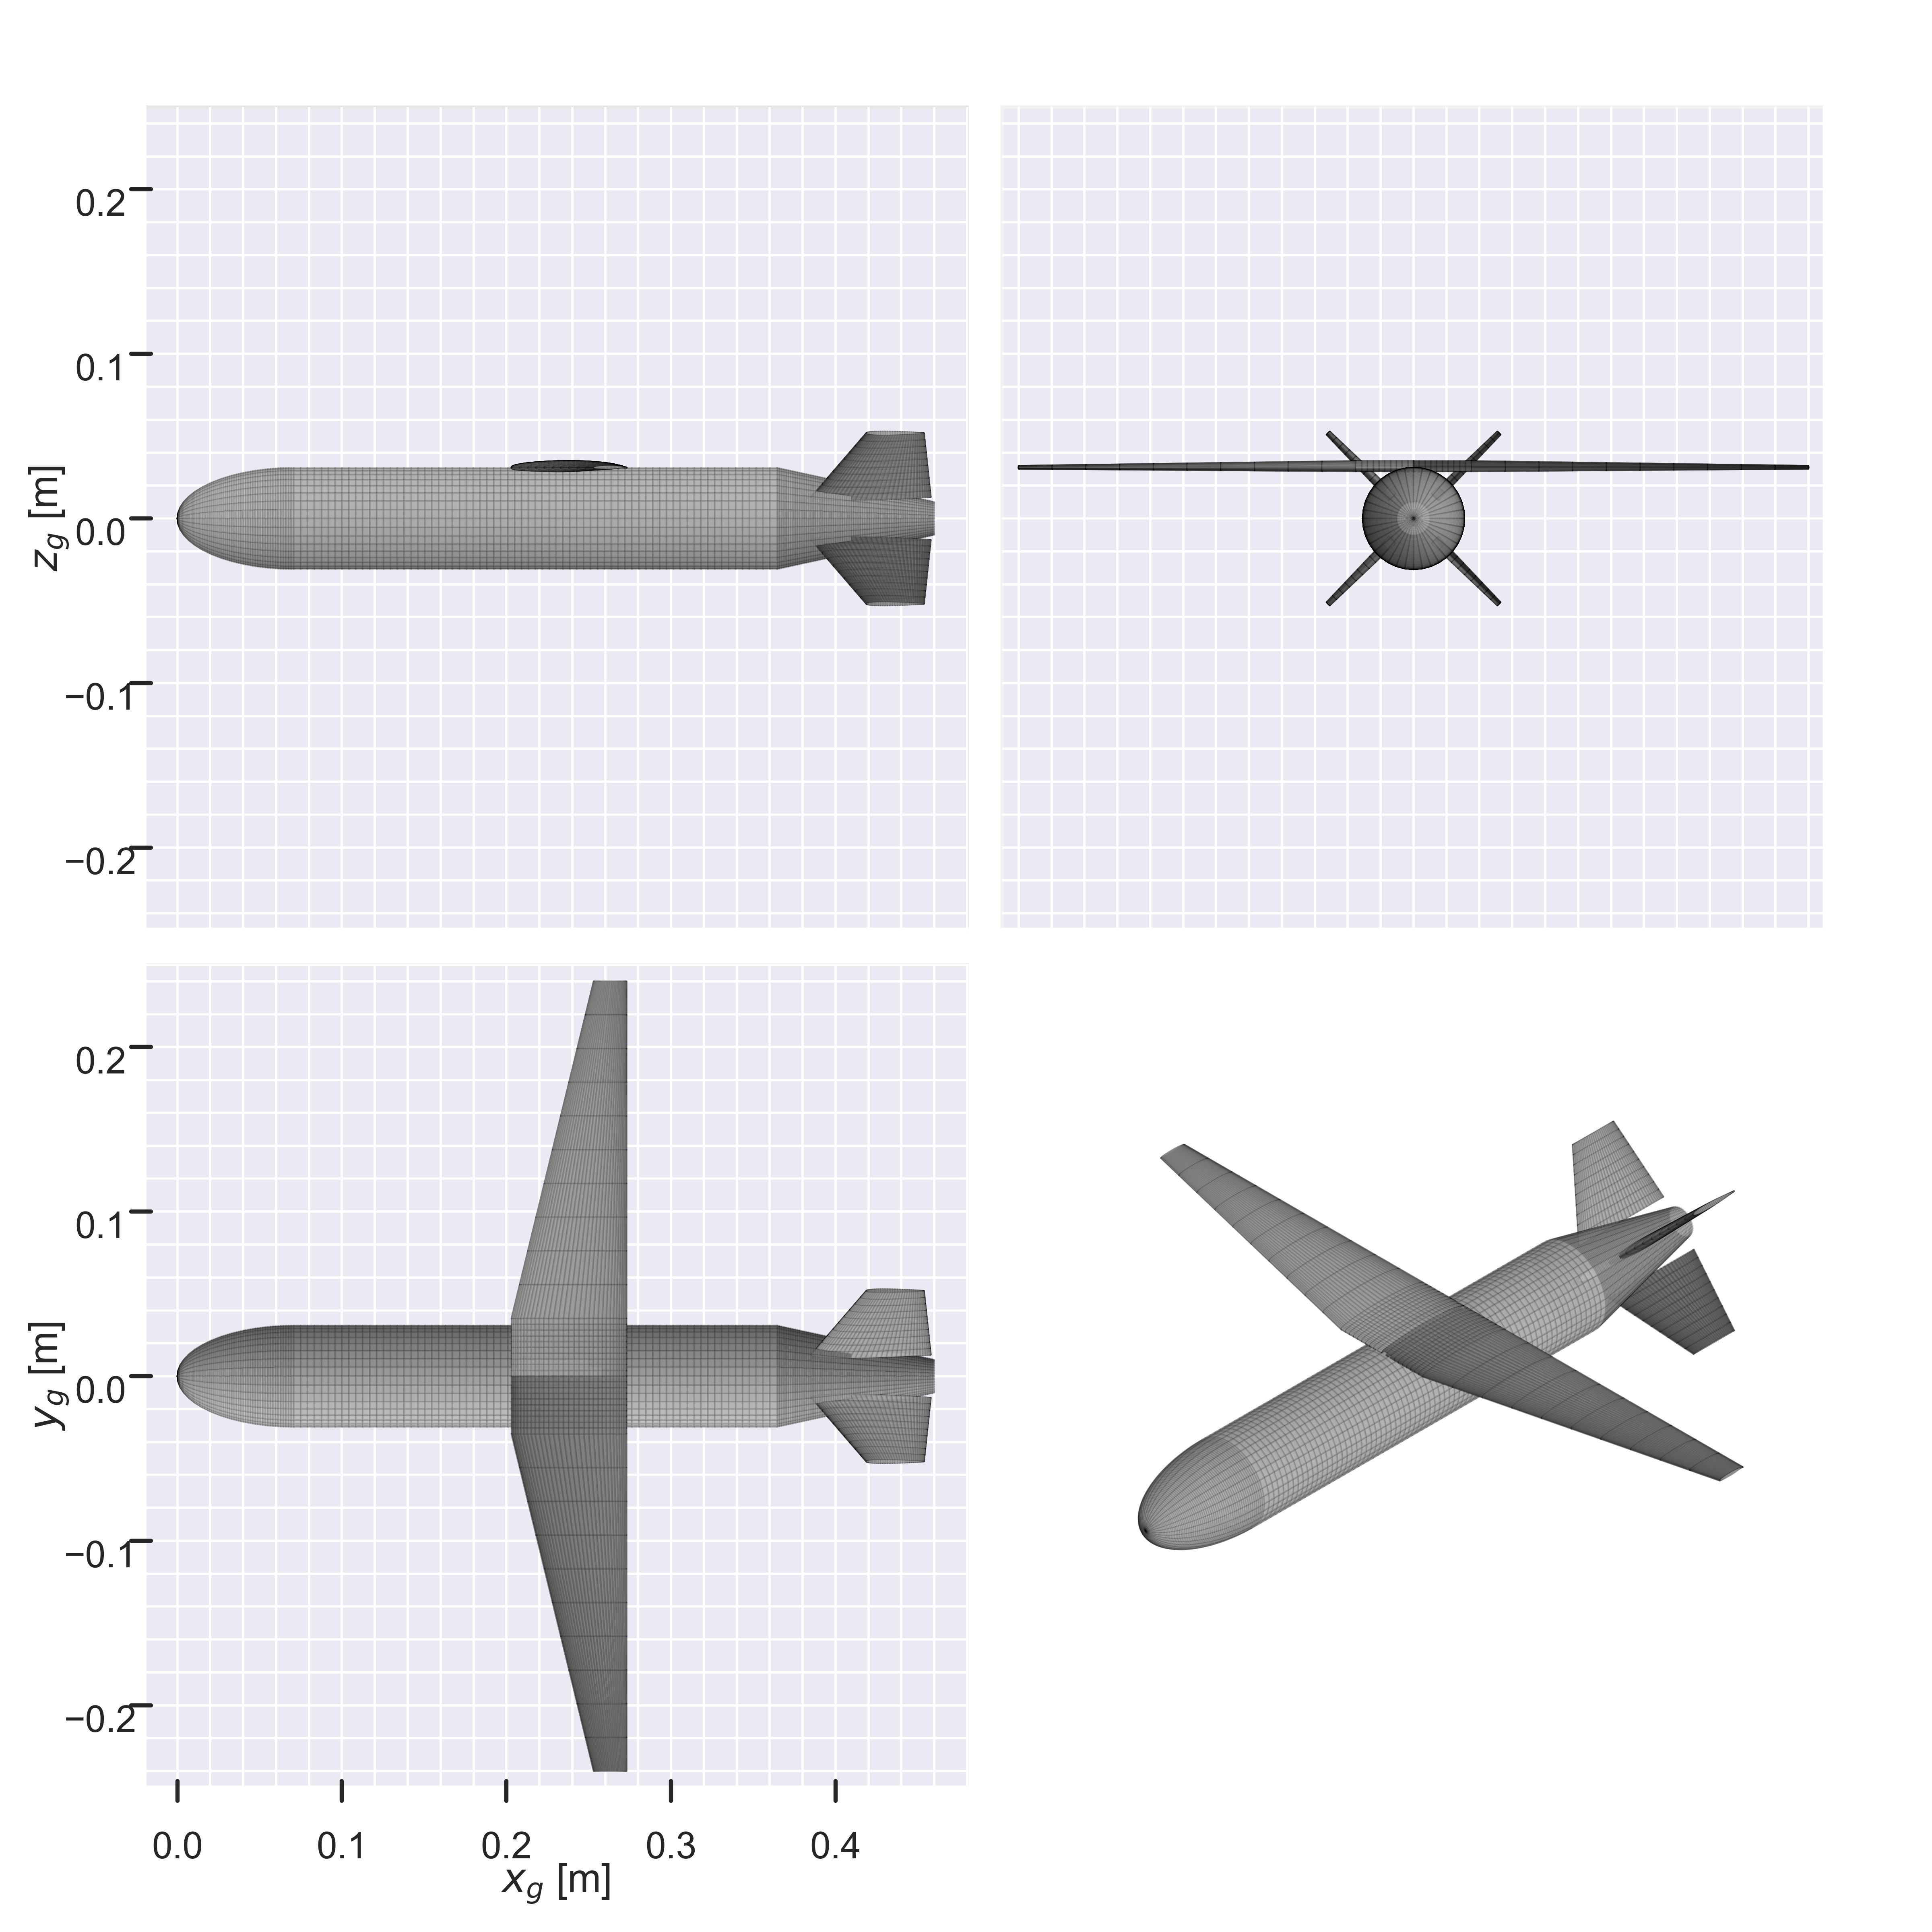
\includegraphics[width=\textwidth]{../figures/firefly_geometry.png}
    \caption{Raw user-facing output of the AeroSandbox geometry stack for the MIT Firefly UAV.}
    \label{fig:firefly_geometry}
\end{figure}

Internal volume and mass accounting of various components at the design point are shown in Table \ref{tab:firefly_mass}, with values that were later validated against as-built prototypes.

\begin{table}
    \centering
    \caption{Mass and volume accounting of various components of the MIT Firefly UAV, at the point design resulting from the formulation given in Section \ref{sec:firefly-mdo}. Mixed units are the result of preferences by various project stakeholders.}
    \label{tab:firefly_mass}
    \begin{tblr}{
        colspec={@{} l m{4cm} m{4cm} m {4cm} @{}},
        row{1}={font=\bfseries},
        column{1}={font=\bfseries},
    }
        \toprule
        Component         & Internal volume [$\rm in^3$] (Percentage) & Mass [gram] (Percentage of gross) & $x_g$ of CG, relative to nose datum [mm] \\
        \midrule
        Fuel (at gross)   & 38.8 (54.2\%)                             & 1019 (42.7\%)                     & 321                                      \\
        Battery           & 9.8 (13.7\%)                              & 322 (13.5\%)                      & 58                                       \\
        Case              & 7.9 (11.0\%)                              & 579 (24.2\%)                      & 230                                      \\
        Liner             & 5.7 (7.9\%)                               & 136 (5.7\%)                       & 321                                      \\
        Mechanisms        & 4.1 (5.8\%)                               & 20 (0.8\%)                        & 447                                      \\
        Payload           & 2.5 (3.5\%)                               & 100 (4.2\%)                       & 78                                       \\
        Avionics          & 2.1 (2.9\%)                               & 75 (3.1\%)                        & 100                                      \\
        Nozzle            & 0.7 (1.0\%)                               & 15 (0.6\%)                        & 447                                      \\
        Wing              & -                                         & 53 (2.2\%)                        & 188                                      \\
        Tails             & -                                         & 70 (2.9\%)                        & 436                                      \\
        \midrule
        Total (gross)     & 71.5 (100\%)                              & 2389 (100\%)                      & 248                                      \\
        Total (zero-fuel) & 71.5 (100\%)                              & 1370 (57.3\%)                     & 195                                      \\
        \bottomrule
    \end{tblr}
\end{table}

The resulting trajectory, which was simultaneously optimized with the vehicle, is shown in Figure \ref{fig:firefly_trajectory}. Here, a number of notable findings can be observed:

\begin{enumerate}
    \item The vehicle is capable of achieving far greater operational range than had been initially anticipated. Initial hand-calculated estimates based on an assumed vehicle design and trajectory had estimated that total ranges of 70 kilometers might be possible\footnote{As a rough napkin-math calculation, a 60-second dash at Mach 0.8, followed by a glide at a $L/D$ of 7 (owing to the low Reynolds number and assumed low-aspect-ratio wing) yields a range of 70 km.}, while the combined optimization result yields ranges of over 230 kilometers.
    \item This massive range increase is achieved partially by co-optimization of various aircraft subsystems, like making aeropropulsive trades on the fuselage shape, which influences dash range. This was expected, and is typical of the power of an MDO approach. However, the majority of the range increase was due to the unique trajectory that the optimizer found, which is shown in Figure \ref{fig:firefly_trajectory}. Here, the vehicle rapidly climbs to a very high altitude—well into the stratosphere—before gliding down. This allows the vehicle to take advantage of two clever effects:
    \begin{enumerate}
        \item The arcing trajectory effectively lets the vehicle use gravitational potential energy as a battery. Because of this, the burn duration of the solid rocket motor can be much shorter for a given impulse, as excess energy goes somewhere useful (i.e., altitude) rather than somewhere wasteful (i.e., wave drag). By allowing a shorter burn, the propellant chemistry can be tweaked to use less burn rate suppressant (oxamide), which increases the specific impulse of the motor. This dynamics-propulsion coupling was not foreseen.
        \item By climbing high, the \emph{indicated} airspeed of the vehicle is much lower while holding the Mach 0.8 constraint. This reduces the dash-phase drag penalty of having a large, high-aspect-ratio, high-$L/D$ wing. By increasing the wingspan, the glide-phase $L/D$ becomes much larger, which gives a large range increase. In addition to enhancing the glide ratio, climbing high also simply increases the glide range directly. This inter-phase aerodynamic trade was also unexpected.
    \end{enumerate}
\end{enumerate}

\begin{figure}[h]
    \centering
    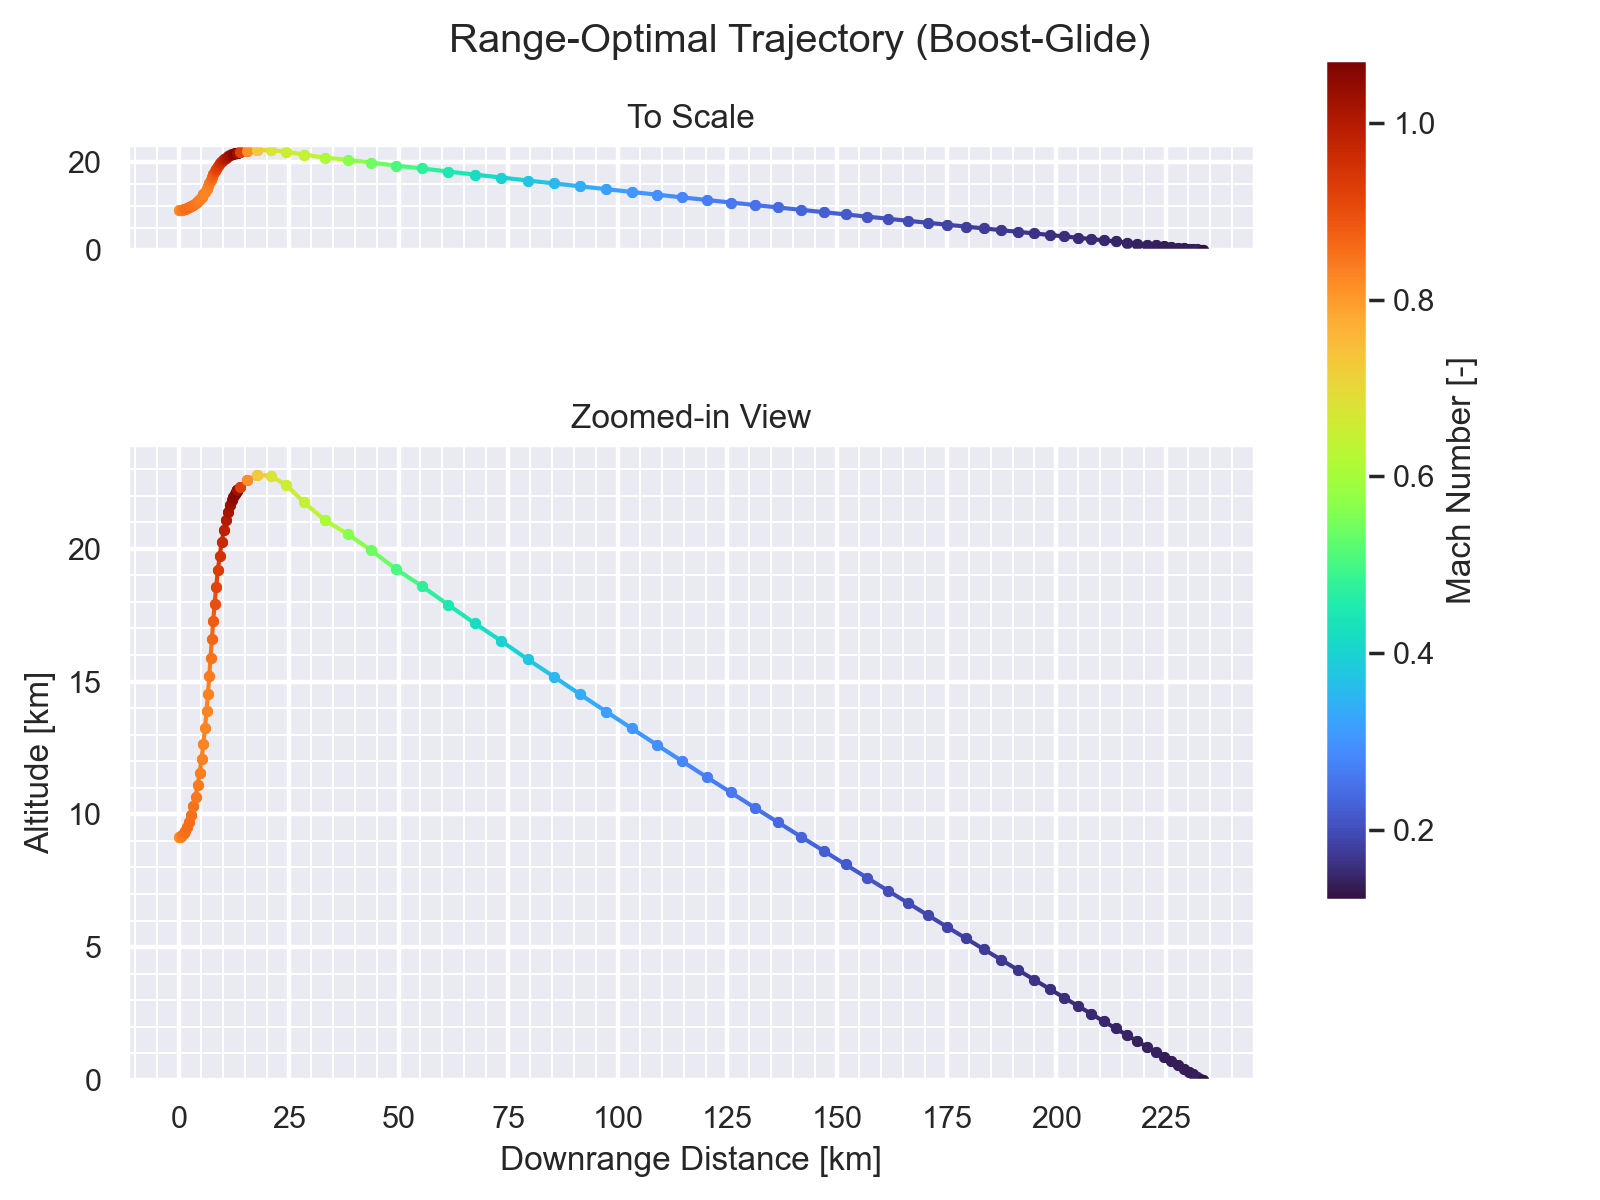
\includegraphics[width=\textwidth]{../figures/BAE-2022-06-17-Peter/ppt/media/image7.png}
    \caption{Trajectory that maximizes vehicle total range, resulting from the combined vehicle-and-trajectory MDO problem formulation given in Section \ref{sec:firefly-mdo}.}
    \label{fig:firefly_trajectory}
\end{figure}

This trajectory, while unexpected, indeed satsifies requirements, and its discovery was only possible through the use of a combined vehicle-and-trajectory optimization approach. This is a key benefit of the code transformations paradigm: the ability to rapidly explore the design space and discover unexpected interactions between subsystems.

\subsection{Design Space Sweeps}

As discussed further in Appendix \ref{appendix:rules-of-thumb}, the value of an engineering design optimization framework is not just in the point design, but also in the insight that it provides. An early example of this observation was made during the Firefly design study, where the optimizer was used to explore the tradeoffs between optimizing for total range (dash + glide) vs. optimizing for dash range alone. In AeroSandbox, this can be easily performed, all without leaving a procedural coding style with the following syntax:

\begin{enumerate}[noitemsep]
    \item Replace the objective function with a simple linear combination of the total and dash ranges, with a weighting factor $w \in [0, 1]$. Define $w$ as an optimization parameter, using:
    \begin{minted}[highlightlines={5}]{python}
        import aerosandbox as asb
        opti = asb.Opti()  # Initialize an optimization environment
        ... # Define the rest of the optimization problem

        w = opti.parameter()
    \end{minted}

    \item Instead of solving the problem with \mintinline{python}{opti.solve()}, solve it with:

    \begin{minted}[highlightlines={1}]{python}
        sols = opti.solve_sweep({w: np.linspace(0, 1)})
    \end{minted}

\end{enumerate}

Using this syntax, the user can convert a point design optimization problem to a design sweep (i.e., looking at a set of optimal points, as some parameter is varied) in just two lines of code.

For this particular case study, the results of such a sweep are shown in Figure \ref{fig:firefly_pareto}. Clearly, though designs can be optimized purely for total range or only for dash range, there are many opportunities where a small sacrifice in one can yield large gains in the other—this may be of interest to the practical designer. Likewise, it shows how the vehicle resulting from the optimizer (in the lower-right) differs dramatically from the original napkin-math ``mental model'' that was used for initial performance estimates. Because this initial design did not use an arcing trajectory, the wing area (and hence, glide-phase $L/D$) was quite limited.

Charts like these can be crucial in high-level conceptual decisionmaking, where an entire family of aircraft can be depicted in a single chart. The results of this design sweep take a few minutes to compute in serial, but parallelization across cores or computers can allow this to be presented to the user in seconds.

\begin{figure}[h]
    \centering
    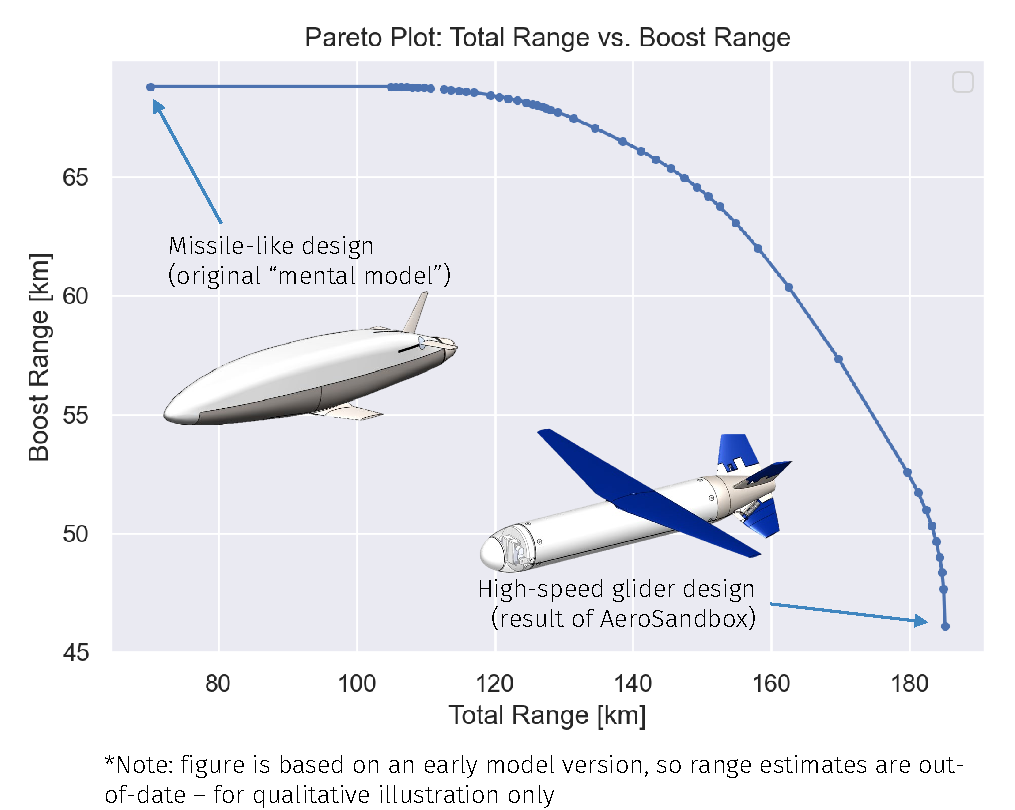
\includegraphics[width=\textwidth]{../figures/firefly_pareto-crop.pdf}
    \caption{Pareto front of the MIT Firefly UAV design space, showing the tradeoff between total range and dash range. Each point represents both a unique vehicle design and trajectory.}
    \label{fig:firefly_pareto}
\end{figure}

\subsection{Supporting Flight Test}

Finally, AeroSandbox-based performance calculations were used to support the Firefly air vehicle through manufacturing, first flight, and a controls characterization flight test campaign \cite{gaubatz_design_2024}. Media from this flight test campaign are given in Figure \ref{fig:firefly_flight_test}. The vehicle was found to be stable and controllable, and the flight test data was used to validate the aerodynamics model used in the optimization problem.

This experience emphasized how useful it is to have an MDO tool that can switch between analysis (e.g., only closure, no optimization) and design modes, as discussed in the birds-eye view of optimization shown in Figure \ref{fig:birds_eye_view}. An MDO tool, if built correctly, has the potential to follow the vehicle through its lifecycle similar to a digital twin, providing value from the conceptual design phase through to flight test.

\begin{figure}[h]
    \centering
    \begin{subfigure}[b]{0.5\textwidth}
        \centering
        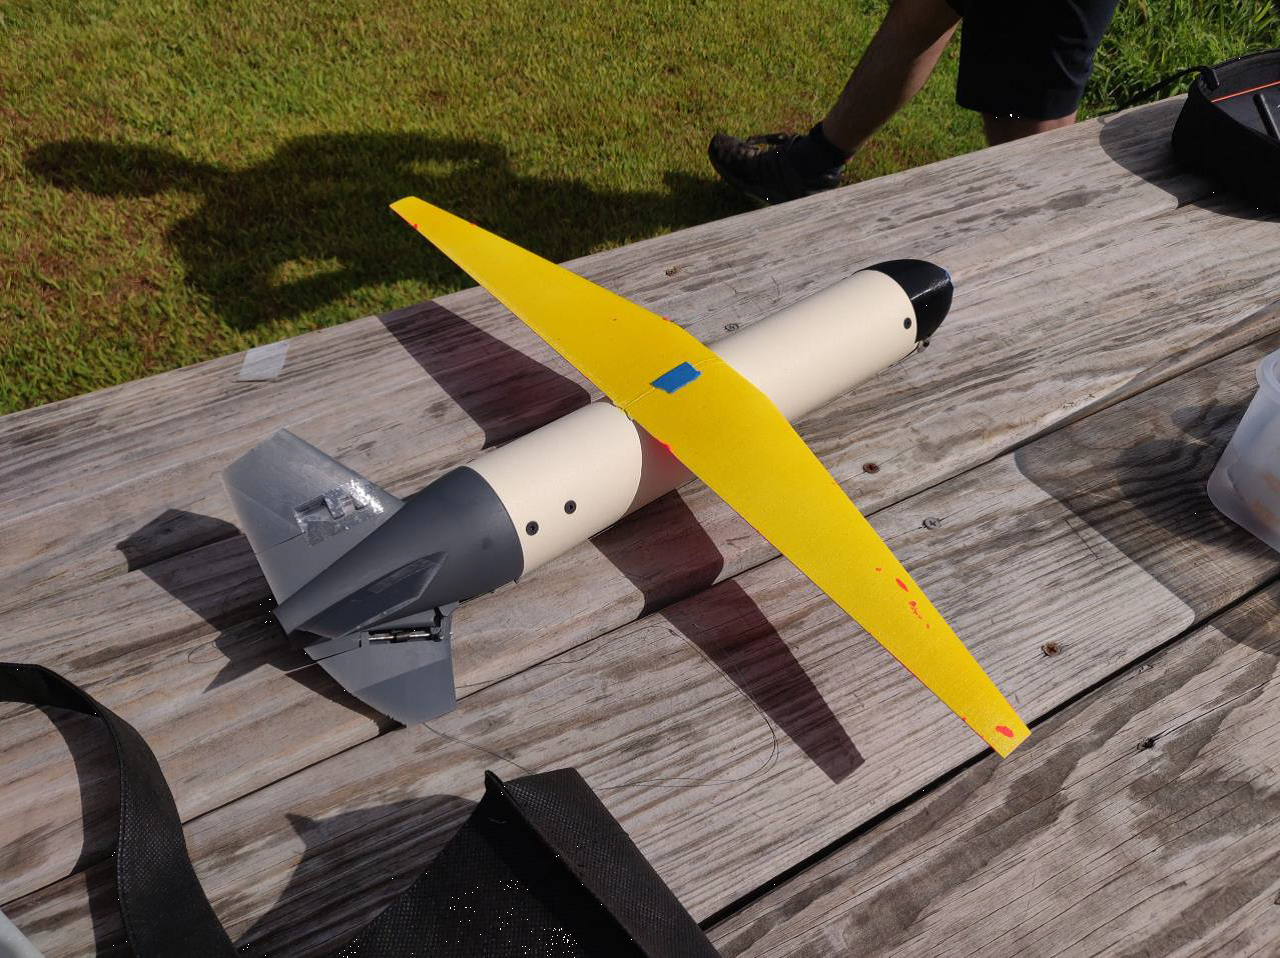
\includegraphics[width=\textwidth]{../figures/firefly_flight_1.png}
        \caption{As-built Firefly air vehicle, prepared for first flight.}
    \end{subfigure}
    \hfill
    \begin{subfigure}[b]{0.432\textwidth}
        \centering
        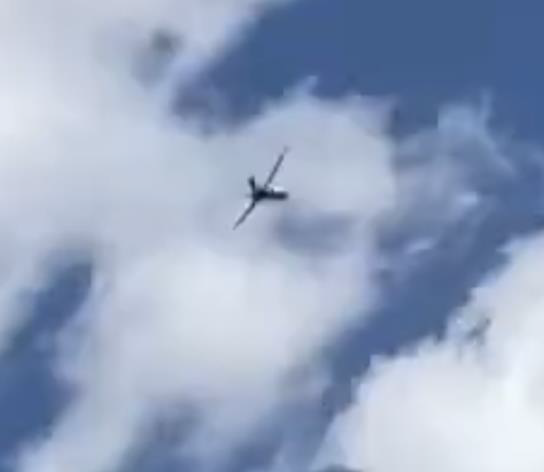
\includegraphics[width=\textwidth]{../figures/firefly_flight_2.png}
        \caption{Photograph of the MIT Firefly air vehicle in-flight, cruising at roughly 40 m/s.}
    \end{subfigure}
    \caption{Photos of the MIT Firefly prototype. Vehicle constructed by Julia Gaubatz \cite{gaubatz_design_2024}.}
    \label{fig:firefly_flight_test}
\end{figure}

\section{Dawn} % TODO name
\label{sec:dawn}

% Grab an XDSM from paper


\section{Hydrogen} % TODO name
\label{sec:hydrogen}


\section{Solar Seaplane} % TODO name
\label{sec:solar-seaplane}


%\section{Other Case Studies} % TODO name
